\documentclass[11pt]{article}
\usepackage{amsmath, amssymb}
\usepackage{geometry}
\geometry{margin=1in}
\usepackage{fancyhdr}
\usepackage{lastpage}
\usepackage{parskip} % Better paragraph spacing
\usepackage{titlesec} % Better section formatting
\usepackage{graphicx}
\usepackage{float}
\usepackage[most]{tcolorbox}
\usepackage{lmodern}
\usepackage{caption}
\usepackage{hyperref}

% Define commands for reusable content
\newcommand{\coursename}{COM-402 Information Security and Privacy}
\newcommand{\lecturenum}{06}
\newcommand{\lecturedate}{\today}
\newcommand{\professor}{Mathias Payer}

\hypersetup{colorlinks=true,linkcolor=blue,urlcolor=blue}

% Configure section spacing
\titlespacing*{\section}{0pt}{2ex plus 1ex minus .2ex}{1.5ex plus .2ex}
% Header / Footer
\pagestyle{fancy}
\fancyhf{}
\fancyhead[L]{\coursename}
\fancyhead[R]{Lecture \lecturenum}
\fancyfoot[L]{EPFL - Computer Science}
\fancyfoot[C]{Author: Jonathan Dutoit}
\fancyfoot[R]{Page \thepage\ of \pageref{LastPage}}

\begin{document}

\begin{center}
  {\large EPFL - Computer Science} \\[0.5em]
  {\Large \textbf{\coursename}} \\[0.5em]
  {\large Lecture \lecturenum\ --- \lecturedate} \\[0.5em]
  {\large Author: Jonathan Dutoit} \\[0.5em]
  {\large Professor: \professor} \\[0.5em]
\end{center}

\vspace{2cm}

\begin{center}
  {\LARGE \textbf{Web and Software Bugs}}
\end{center}

\vspace{0.5cm}

\section*{Learning goals}
\begin{itemize}
	\item Web applications and regular application have a lot in common
	\item Understand the impact of preprocessing attacker-controlled data
	\item Differentiate between types of bugs and what potential attacks they enable
\end{itemize}

\vspace{0.5cm}

\vspace{0.5cm}

\begin{center}
  {\LARGE \textbf{Web Application Security}}
\end{center}
\vspace{0.5cm}

Open Web Application Security Project (OWASP)

Top 10: Common Vulnerabilities 

\textcolor{blue}{Goal: }\textbf{Achieving arbitrary code execution}
\begin{itemize}
	\item Cross-Site Scripting (XSS): Executing JavaScript code
	\item SQL Injection: Executing SQL code
	\item LDAP Injection: Executing LDAP queries
	\item Command Injection: Executing shell commands
\end{itemize}

The \textbf{Top 10} project documents the 10 most critical security risks to web apps. Updated frequently (last update was 2021) and has cross-references to CWEs (Common Weakness Enumeration).

\begin{itemize}
	\item \textbf{A01 Broken Access Control}: Access control enforces policy such that users cannot act outside of their intended permissions. Failures typically lead to unauthorized information disclosure, modification, or destruction of all data or performing a business function outside the user's limits
		\begin{itemize}
			\item CWE-200: Exposure of Sensitive Information to an Unauthorized Actor \\
			  CWE-201: Insertion of Sensitive Information Into Sent Data, and \\
			  CWE-352: Cross-Site Request Forgery
			\item Reduce attack surface by "deny by default"
			\item Implement access control mechanisms once, reuse through app (user session)
			\item Log access control failures
			\item Rate limit API calls
			\item \textbf{Real world example}: Accessing everyone's Google Drive files with Google Classrooms. 
		\end{itemize}
	\item \textbf{A02 Cryptographic Failures}: The first thing is to determine the protection needs of data in transit and at rest. For example, passwords, credit cards numbers, health records, personal information, and business secrets require extra protection.
		\begin{itemize}
			\item CWE-259: Use of Hard-coded \textbf{\textit{"default"}} Password, \\
			  CWE-327: Broken or Risky Crypto Algorithm, and \\
			  CWE-331: Insufficient Entropy
			\item Reduce attack surface by storing minimal data
			\item Ensure up-to-date algorithms and implementations
			\item Disable legacy protcols
		\end{itemize}
	\item \textbf{A03 Injection}: Code injection is possible when attacker controlled data is handled incorrectly and ends up being parsed as code
		\begin{itemize}
			\item CWE-79: Cross-site Scripting, \\
			  CWE-89: SQL Injection, and \\ 
			  CWE-73: External Control of File Name or Path
			\item Reduce attack surface by shifting to safe API
			\item Sanitize user input through validation and escaping
			\item Validate input whenever possible
			\item Escape remaining characters when necessary
		\end{itemize}
	\item \textbf{A04 Insecure Design}: Insecure design is a broad category representing different weakness, expressed as "missing or ineffective control design"
		\begin{itemize}
			\item CWE-209: Generation of error message containing sensitive information, \\
			  CWE-256: Unprotected Storage of Credentials, \\
			  CWE-501: Trust Boundary Violation, and \\
			  CWE-522: Insufficiently Protected Credentials
			\item Prevent by establishing secure development lifecycle
			\item Use threat modeling where feasible
			\item Segregate and compartmentalize where possible
		\end{itemize}
	\item \textbf{A05 Security Misconfiguration}: Software is getting more configurable and administrators need to carefully balance features and security. Any software along a complex stack can be misconfigured.
		\begin{itemize}
			\item CWE-16: Configuration and \\
			  CWE-611: Impostor Restriction of XML External Entity Reference
			\item Document the software stack and its configuration
			\item Harden all configuration
			\item Minimize exposed features
		\end{itemize}
	\item \textbf{A06 Vulnerable / Outdated Components}: Software may have known vulnerabilities that can be abused by an attacker. 
		\begin{itemize}
			\item CWE-1104: Use of Unmaintained Third-Party Components
			\item Minimize attack surface by removing or disabling unused components
			\item Track inventory of software and follow upstream security notices
			\item Monitor for available patches, if patching is not possible mitigate through firewall or high-level interception
		\end{itemize}
	\item \textbf{A07 Identification / Authentication Failures}: Confirmation of the user's identity, authentication, and session management is critical to protect against authentication-related attacks
		\begin{itemize}
			\item CWE-297: Improper Validating of Certificate with Host Mismatch, \\
			  CWE-287: Improper Authentication, and \\
			  CWE-384: Session Fixation
			\item Reduce attack surface through 2FA
			\item Check for good password hygiene (length, weak passwords, policies)
			\item Limit or increasingly delay failed login attempts
		\end{itemize}
	\item \textbf{A08 Software and Data Integrity Failures}: Software and data integrity failures relate to code and infrastructure that does not protect against integrity violations. An example of this is where an application relies upon plugins, libraries, or modules from untrusted sources, repositories, and content delivery networks (CDNs)
		\begin{itemize}
			\item CWE-829: Inclusion of Functionality from Untrusted Control Sphere, \\
			  CWE-494: Download of Code Without Integrity Check, and \\
			  CWE-502: Deserialization of Untrusted Data
			\item Mitigate by verifying (through signatures) that data comes from verified source and has not been tampered
			\item Review code and configuration changes to limit potential mistakes
		\end{itemize}
	\item \textbf{A09 Security and Logging Monitoring}: Breaches will happen. Document ongoing security activities and safely log actions to enable detection and analysis of breaches. 
		\begin{itemize}
			\item CWE-778: Insufficient Logging, \\
			  CWE-117: Improper Output Neutralization for Logs, \\
			  CWE-223: Omission of Security-relevant information, and \\
			  CWE-532: Insertion of Sensitive Information into Log File
			\item Mitigate by logging failed logins, authentication, or access control checks
			\item Ensure high-value transactions have an audit trail
			\item Protect log data through integrity or other safeguards
		\end{itemize}
	\item \textbf{A10 Server Side Request Forgery}: SSRF flaws occur whenever a web application is fetching a remote resource without validating the user-supplied URL. It allows an attacker to coerce the application to send a crafted request to an unexpected destination, even when protected by a firewall, VPN, or another type of network access control list (ACL). 
		\begin{itemize}
			\item CWE-918: Server-Side Request Forgery (SSRF)
			\item Added due to community vote (not observed attack data)
			\item Prevent by implementing defense in depth
			\item Deny by default, sanitize and validate all user data based on allow-list
		\end{itemize}
\end{itemize}

\textbf*{OWASP Top 10 Follow Trends}

% Quick centered image
\begin{figure}[H]
    \centering
    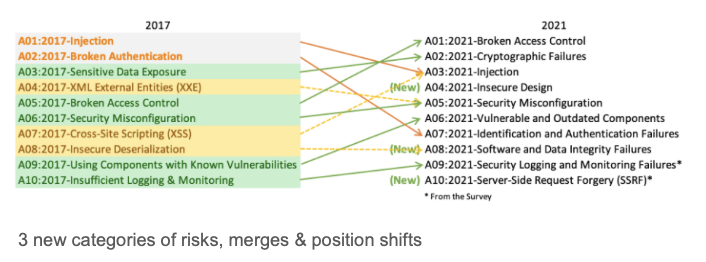
\includegraphics[width=1\textwidth]{top-10-trends}
    \label{fig:LABEL}
\end{figure}

\section*{Arbitrary Code Execution}

Code injection is possible when user-supplied data escapes control. The vulnerability comes from special characters in \textbf{user inputs} can trigger an action in the context (HTML, SQL, LDAP, OS commands, XML, XSL, SMTP).

The impact is an attacker-controlled data becomes code that may be abused to escape the intended behavior of the original code. 

Recent example: Log4j Exploit used in many java-based applications.

\textbf{Protection against Injection}

Deny by default, otherwise inspect received data \textbf{twice}

\textbf{When receiving: Input validation}
\textbf{When using: Encode data}
\begin{itemize}
	\item Escape (encode) special characters when you use them
\end{itemize}

Separate code and data (e.g., SQL prepared statements)

Web frameworks offer sanitization functions! 

For every request, check if the requesting user has adequate permissions!

\vspace{0.5cm}

\begin{center}
  {\LARGE \textbf{Software Security}}
\end{center}
\vspace{0.5cm}

\textbf{threats}
\begin{itemize}
	\item Stack-based overflows 
	\item Direct overwrites through pointer manipulation
	\item Heap-based overflows and overwrites
	\item Underflows instead of overflows
	\item Exception-based hijacking
\end{itemize}

\textbf{Note}: In this lecture we focus more on stack-based/buffer overflows (variable overwrite, overflowing return address, code injection, etc.). More information about software security is given by CS-412 in Spring. 

Programmers are not perfect, all software therefore has bugs. Some bugs make the software vulnerable and sooner or later adversaries will find a way to exploit those vulnerabilities. We make a difference between \textbf{logic bugs} (e.g., forgetting to check access permissions) and \textbf{bugs that violate memory and type safety}, leading to memory corruption.

\textbf{Defense Strategies}

1. \underline{Memory safety}: stop memory corruption by using safe languages (Java/Rust)

2. \underline{Integrity}: enforce integrity of reads/writes by doing Write Integrity Testing, Code-Pointer integrity, etc...

3. \underline{Randomization}: Probabilistic defenses by randomizing locations, code, data, or pointer values. 
\begin{itemize}
	\item Oscar made a really good point about Anti-Cheating in games often randomized variable locations so that cheats can't work
\end{itemize}

4. \underline{Flow Integrity}: protect control transfers by verifying data-flow and control-flow integrity.

5. If we cannot assure all steps above, the our program is susceptible to \textcolor{red}{Attack:} Control-flow hijack

\section*{Defense: DEP Hardware Support}

Page table extension, introduce NX-bit (No eXecute bit) which was conceived in the early 2000s following the advancement of operating systems supporting 64-bit architecture instead of only 32 bits. Having a 64-bit architecture allowed space for the DEP. 

This is an additional bit for every mapped virtual page. If the bit is set, then data on that page cannot be interpreted as code and the processor will trap if control flow reaches that page. 

\section*{Defense: Address Space \textbf{Layout} Randomization (ASLR)}

ASLR is a \textbf{pratical form} of Address Space Randomization. It focuses on blocks of memory (i.e., it is coarse grained). 

Heap, stack, code, executable, mmap regions end up at random addresses. 

ASLR is inherently page-based, limiting cost of shuffling and it initializes when process starts (never re-randomized). It can also be combined with DEP for better security. 

\section*{Defense: Stack Canaries}

Early attacks overflowed stack-based buffers to inject code. Memory safety would mitigate this problem but adding full safety checks is infeasible due to high performance overhead. 

Instead of checking each pointer dereference, check integrity only before important data is accessed, e.g., before accessing a code pointer. 

\textbf{Assumption}: we only prevent RIP (return instruction pointer) control-flow hijack attacks. 

Therefore, only need to protect the integrity of the RIP. Key insight: buffer overflows are only possible after pointer arithmetic. 

Hence, the strategy is to place a canary after a potentially vulnerable buffer and after check the integrity of the canary before the function returns. 

Limitation: the stack canary only protects against \textbf{\textit{continuous overwrites}} if (and only if) the attacked does not know the canary. An alternative is to encrypt the return instruction pointer by xoring it with a secret

Hence, Canary is stored in a safe location, copied to stack slot in prologue and checked in epilogue before returning. It protects against most stacked-based hijack attacks and it's simple, low-overhead compiler-based defense. 
\end{document}

